\documentclass[conference]{IEEEtran}
\IEEEoverridecommandlockouts
% The preceding line is only needed to identify funding in the first footnote. If that is unneeded, please comment it out.
\usepackage{cite}
\usepackage{amsmath,amssymb,amsfonts}
\usepackage{algorithmic}
\usepackage{graphicx}
\usepackage{textcomp}
\usepackage{xcolor}

\def\BibTeX{{\rm B\kern-.05em{\sc i\kern-.025em b}\kern-.08em
    T\kern-.1667em\lower.7ex\hbox{E}\kern-.125emX}}
\begin{document}

\title{Blind Assistance System using an FPGA\\
\thanks{Identify applicable funding agency here. If none, delete this.}
}

\author{\IEEEauthorblockN{Omkar Nandan Choudhary}
\IEEEauthorblockA{\textit{Department of Electronics} \\
\textit{TCET}\\
City, Country \\
email address or ORCID}
\and
\IEEEauthorblockN{Ishaan Shinde}
\IEEEauthorblockA{\textit{Department of Electronics} \\
\textit{TCET}\\
City, Country \\
email address or ORCID}
\and
\IEEEauthorblockN{Arun Kumar Singh}
\IEEEauthorblockA{\textit{Department of Electronics} \\
\textit{TCET}\\
City, Country \\
email address or ORCID}
}

\maketitle

\begin{abstract}
Sighted guidance is arguably the most efficient way of guiding the
visually impaired. Sighted guidance system will provide haptic
feedback to the user about the obstacles in the user's path. To detect
these obstacles, different options are available for sensors. Among
these we are using a stereo camera to take advantage of its ability to
provide visual information about the user's surrounding and ultrasonic sensors placed strategically to estimate the distance between the user and the obstacle. This data is run
through a YOLO based algorithm which will be trained to detect
obstacles in the user's path and this will be relayed back to the user
using Haptic feedback. The FPGA can provide true parallel processing while maintaining
reconfigurability and programmability. This sensors will be mounted
on a standard white cane, reason being this piece of equipment is
already familiar and a part of the daily life for the visually impaired. This system will inform the user about obstacles in 5-8
meters range and will allow them to navigate around these obstacles
easily and safely.
\end{abstract}

\begin{IEEEkeywords}
Blind Assistance, FPGA, YOLO, Object Detection.
\end{IEEEkeywords} 

\section{Introduction}
Around 62 million people in India are visually impaired, for them performing even basic daily tasks is a challenge. An activity as simple as travelling, which is one of the most fundamental parts of our daily life, can become a havoc. Walking in an urban environment means there are several obstacles in the path, these may be fellow travellers, stray animals or some other obstacles. Navigating around these obstacles can be a problem for the visually impaired. Such inconveniences in travelling disrupts their daily life. This project aims to provide a solution for these issues faced by them.We focus our project on helping them navigate while walking. To do this, we are reinforcing the already in use walking stick used by them. We are planning to design a system which will be mounted on this stick and will enable them to micro-navigate in situations where relying only on a regular walking stick is not feasible. This system will see the path in front and will try to identify potential obstacles in the path and inform the user using haptic feedback. This will help them preemptively judge the surrounding layout and the approximate location of obstacles. Doing this will make it easier for them to travel and will save effort and time. 

\section{Literature Review}

Based on reports from WHO, the estimated count of visually impaired individuals in India is around 62 million. Since the year 2000, the count of visually impaired individuals has seen a steep rise across the years. This type of predicament makes it difficult for such individuals to survive normally without any external assistance. Over the years such assistance was provided by physical helpers such as a medical assistant, a pet, a relative, walking aids (such as a cane), etc. However, these types of assistance generally put a degree of dependence on other humans for the visually impaired individuals to perform even basic tasks. It is of utmost importance to innovate in the field of smart assistance for blind individuals as they add up to a large amount of the population of the country. As a part of our literature survey for the project, a range of designs were reviewed. For our project, due consideration of all the previously done research is made and a solution has been proposed accordingly.\newline
\newline[1].Smart Cane for Blind and Visually Impaired Persons. Year of Publishing:May, 2020 \newline
\newline The proposed work includes the design of a smart cane with multiple sensors connected to an Arduino board. ultrasonic and infrared sensors are mounted at appropriate locations to detect obstacles. A buzzer, vibrator, and some recorded audio clips to navigate the blind people safely.\newline
\newline[2].Design and Implementation of Mobility Aid for Blind People. Year of Publishing:August, 2015 \newline
\newline Draws attention to the shortcomings of already existing solutions. The proposed solution is a Jacket that has to be worn by the visually Impaired. The Jacket is mounted with a collection of ultrasonic Sensors to provide assistance to the user. \newline
\newline[3].Ultrasonic Navigation-based Blind Aid for the Visually Impaired. Year of Publishing:June, 2018
\newline The proposed system operates in two modes namely hurdle detection mode and fixed mode. In this mode, the system detects solid and liquid obstacles sending respective instructions to the blind person through voice messages via Bluetooth. The fixed mode provides the information and guidance to move from one place to another safely by setting a fixed route in blind stick from source to destination location. Additionally, the system uses GPS data, Bluetooth to assist the visually impaired. \newline
\newline[4].Survey on assistance systems and Navigation for Blind People using Sensors. Year of Publishing: January 2018. \newline
\newline A survey paper to understand the most reliable and efficient assistance systems for the visually impaired. \newline
\newline[5].A Stereo Vision System for Pedestrian Navigation. Year of Publishing: 2003. \newline
\newline In this paper, the project was implemented using Stereo cameras. For accurate motion estimation Gait analysis and ego-motion estimation, algorithms are used. \newline
\newline[6].A system for remote sighted guidance of visually impaired pedestrians. Year of Publishing: 2003. \newline
\newline In this paper, the authors designed the guidance system using GPS as the main navigation device. As shown in the paper the accuracy of this approach is not sufficient enough for users to be able to traverse an unknown path with ease. This is especially true in cases where obstacles are blocking the GPS signal. They have also proposed to use cameras to supplement the GPS device.


\section{Research Gaps}
The primary aim of this project is to develop a product to cater to visually impaired individuals in the Indian environment. However, the ergonomics of the final product needs to be optimized considering the ease and comfort of the end-user. The position of the sensors and the location of the final product will be of critical importance. The ease of use needs to be a priority when designing a device for the visually impaired. The device's power consumption should be optimized and justifiable, considering the hardware used and services provided to the end-user. Battery Pack of the right chemical composition and specifications should be incorporated to optimize battery health and minimize the re-charge frequency. The device should be easily tune able by the end-user and he/she should not require external assistance to use the device or modify its operation.

\section{Ergonomics}
Over the years, a variety of innovations have come forward to cater to the visually impaired population. Some required the user to wear it on their upper body, eyewear, headgear, footwear, etc., or a combination of mentioned locations. Most of these mentioned solutions had their unique advantages and disadvantages. However, it was observed that most of these assistance devices required the end-user to adopt a completely new or different way of getting assistance. This process of learning and understanding the requirements of the assistant device takes time and effort from the end-user. It would be only correct if we think of providing assistance to such individuals that involve an item already familiar to them and thus requires less time and effort from the end-user. Here, we have presented an idea that provides the visually impaired individuals with a device that revolves around an object that they are familiar with, a walking cane. The target individuals are very familiar with the utility of a walking cane, most individuals also hold preliminary training on how to use a walking cane already. A smart walking cane that has a combination of sensors mounted on it to acquire the surrounding data can be used to provide the user with the necessary data and suggestions. Sensors such as a visual sensor (stereo camera) and an ultrasonic/IR Sensor for distance estimation between the user and an object in the path will be mounted on the cane. The received data will be sent to the main processing unit to then provide the user with the necessary suggestions. The primary reason behind selecting vibrations as a medium of providing feedback to the user is because from research over the years it has been found that people who have a visual disability by birth or develop It later due to various reasons have an enhanced sense of hearing and touch or at least rely more on their other senses to get an understanding of their surroundings. They are naturally better at identifying the source of any noise or any sound than any regular person could otherwise, and disrupting this by making the user wear an earphone or headwear for an audio alerts system might hamper the natural ability of the person. The incorporation of a walking cane as a solution would also make it conspicuous to the fellow pedestrians about the user's condition and suggest them to remain alert or cautious in case of any emergency or misshaping.

\begin{figure}[htbp]
\centerline{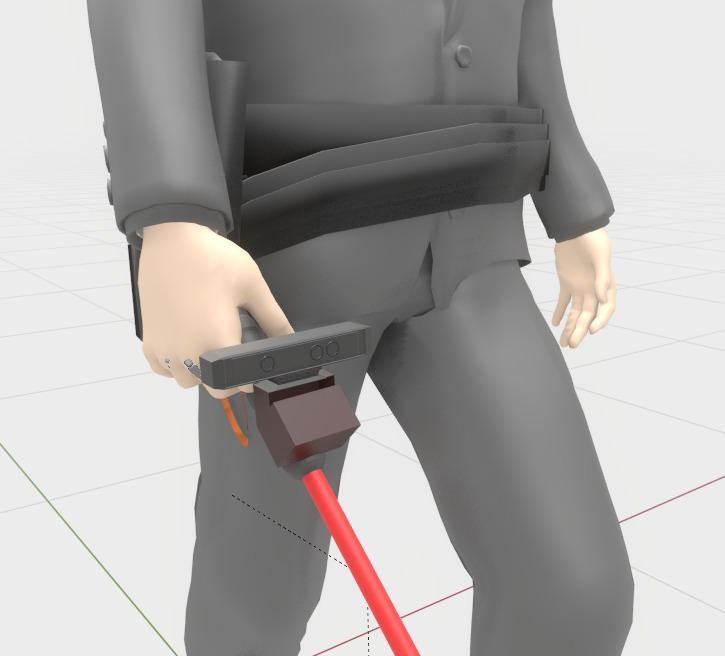
\includegraphics[scale=0.25]{blender-camera.jpeg}}
\caption{Camera and Zigbee transmitter.}
\label{fig}
\end{figure}

\section{Methodology}\label{SCM}
In this project, the combination of a Field Programmable Gate Array (or FPGA) and an stereo camera will be explored to get effective data about the surroundings of the user. The medium of haptic feedback will be used to alert the user. A 2V - 5V dc mini vibration motor will be used. Haptic alerts are considered being one of the most preferred choices in types of feedbacks, as it eliminates the need for the user to wear any extra feedback equipment (like earphones, etc.) which might block or hamper the user’s natural ability of hearing. The Zigbee RF modules will be helpful in establishing communication between the main FPGA processing unit and the RGBD camera. Features of FPGAs like concurrent processing of data provide faster and reliable data at the outputs as compared to that of an Arduino or similar microcontroller boards. The RGB-D camera will be mounted on a general walking cane (for visually impaired), so the user doesn’t need to depend on or learn handling of any new equipment and can perform his or her task of daily commute with ease and assurance.

\begin{figure}[htbp]
\centerline{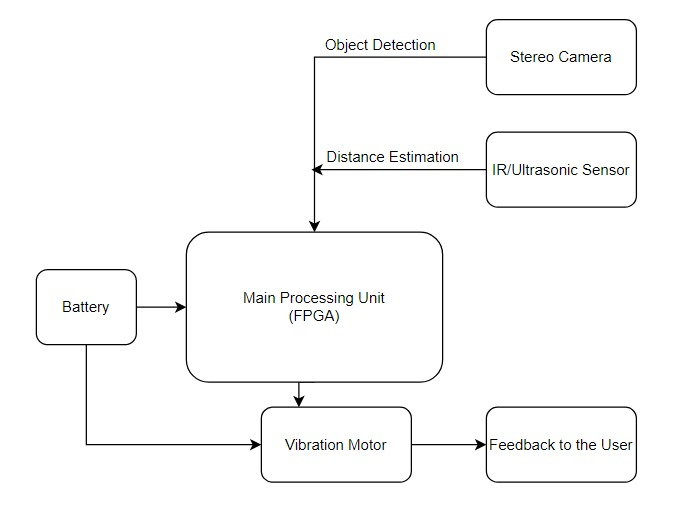
\includegraphics[scale=0.4]{blockdiagram.jpeg}}
\caption{Camera and Zigbee transmitter.}
\label{fig}
\end{figure}

\subsection{Object Detection}\label{AA}
Object detection is handled by YOLOv4, YOLOv4 boasts inproved performance compared to its predecessors in instances of parallel processing. This makes it ideal to be used with an FPGA. YOLO has the added benefit of faster object detection speeds when compared to algorithms such as R-CNN, sliding window and region proposal based techniques \cite{yolo}. 

\subsection{Feedback to the user}
Once the objects are detected they are classified into groups and each group has a different vibration pattern allocated to them. These patterns will help the user understand their environment better. We are organising the objects based on their speed and location compared to the user. These groupings are:
\begin{itemize}
\item Obstacles within 3 meters.
\item dsafasf
\end{itemize}


\bibliography{paper}{}
\bibliographystyle{plain}

\end{document}
